Android OS does not provide any functionality to store or manage tasks. There are several applications available in the market place to fill that void, but unfortunately non of these is suitable for the intended use-case in this project.  The existing solutions do not provide Android Content Providers and the data models used do not provide the functionality needed here. Therefor it was necessary to implement a solution for this problem from scratch.\\\\
In Kangaroo each task is represented by an instance of the class com.kangaroo.task.Task. Each instance has a task name, a description and a unique ID. Also each task keeps a list of constraints. Each task has an arbitrary number of constraint and each constraint limits its execution in a certain way. The following constraints are available, each implements the TaskConstraintInterface:
\begin{itemize}
\item TaskConstraintDate: The task can only be executed between two predefined dates.
\item TaskConstraintDayTime: A task with this constraint can only be executed at a certain time of day.
\item TaskConstraintDuration: The task takes n minutes to perform.
\item TaskConstraintLocation: The task needs to be executed at certain coordinates.
\item TaskConstraintPOI: The task can be executed at points of interest of a certain type, e.g. an ATB or a Bakery.
\end{itemize}
With this functionality a big number of possible tasks can be represented. Additional Constraints can be added at any time, as long as they implement the TaskConstraintInterface.\\
\begin{figure}[h!]
\centering
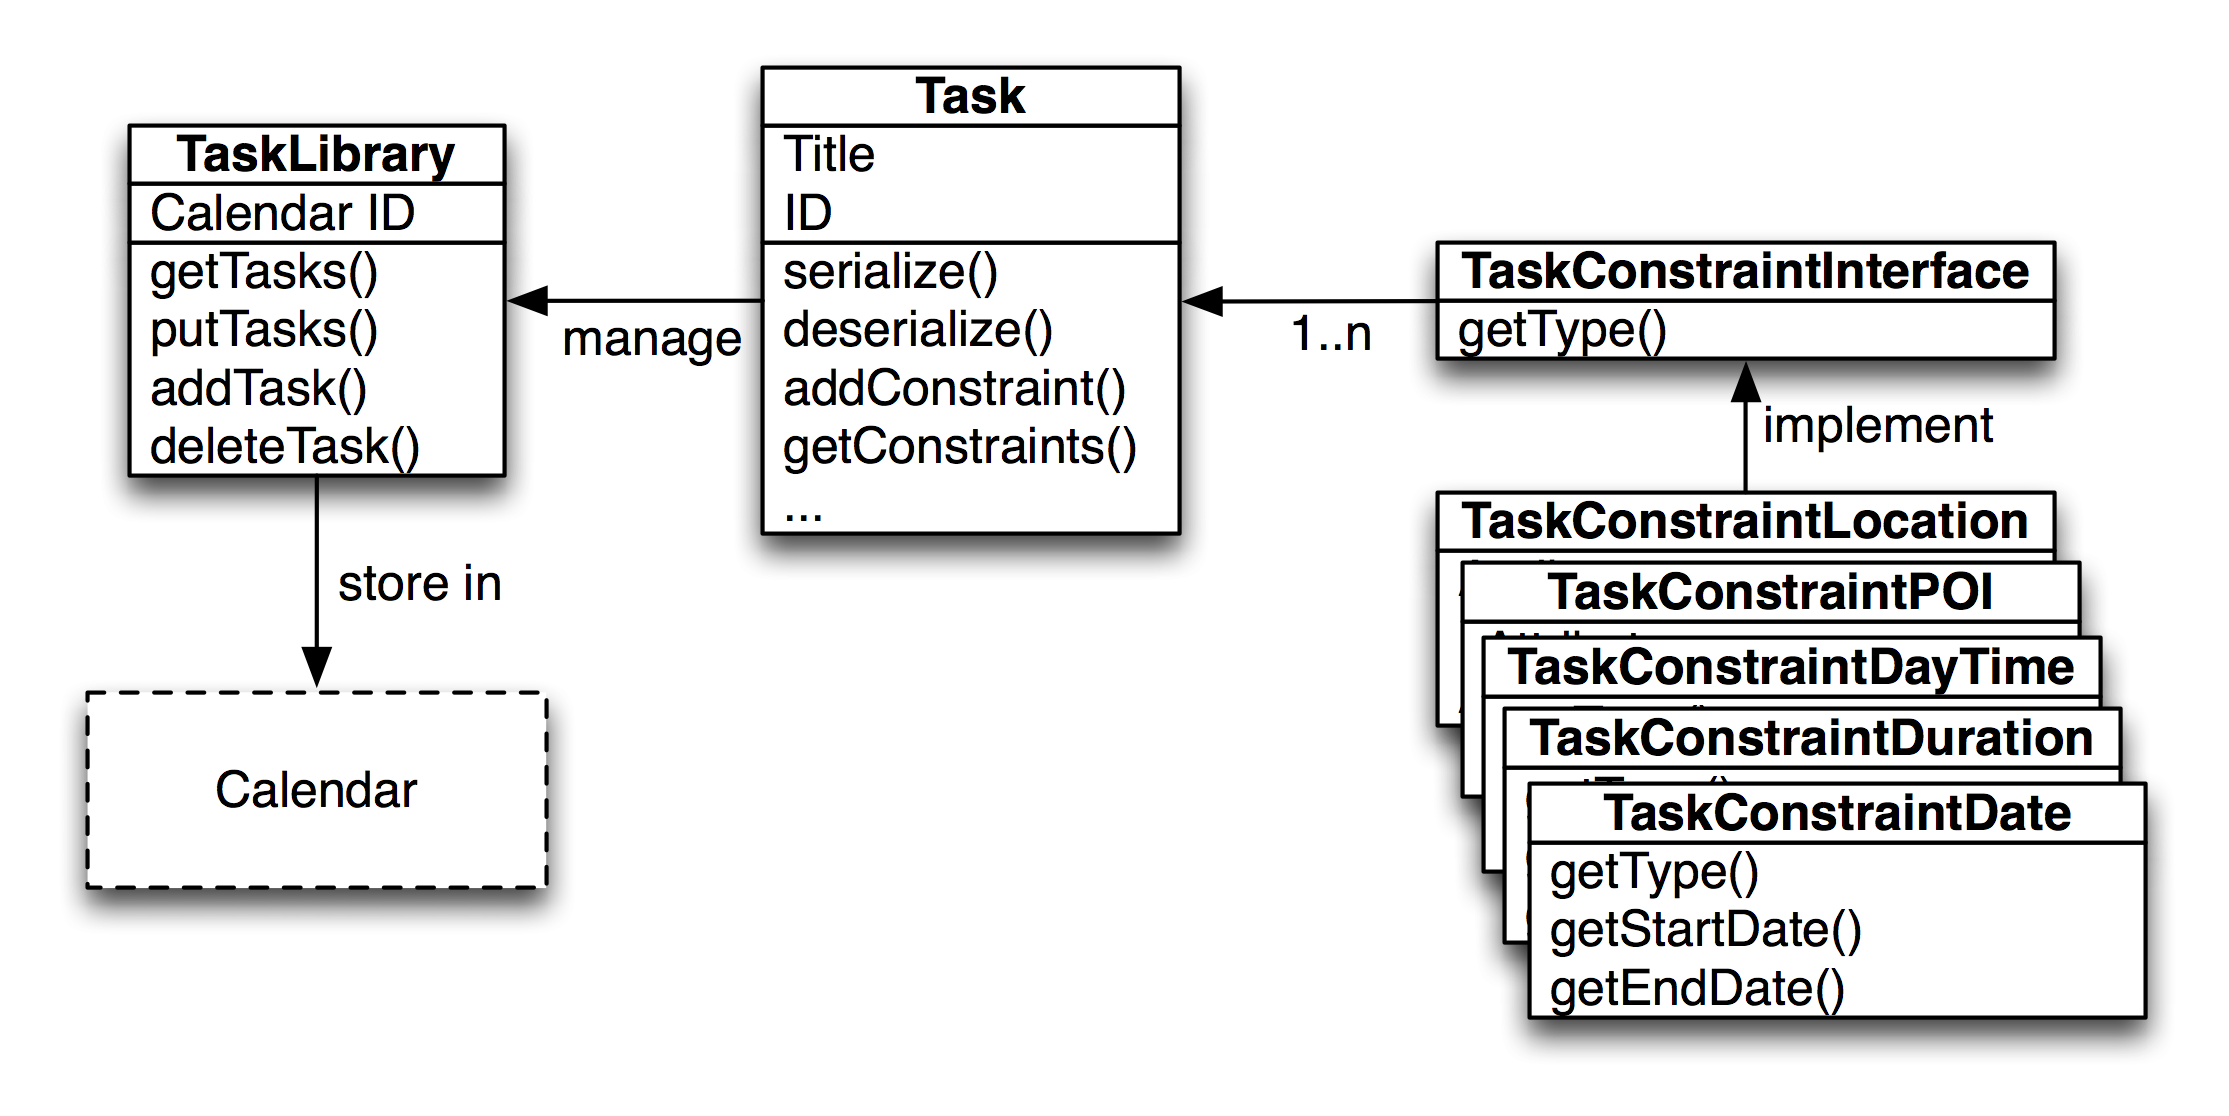
\includegraphics[width=14cm]{pics/task_class.png}
\caption{Diagram of the task-related classes}
\label{task_class}
\end{figure}  
Obviously the list of tasks needs to be persistent, even when the application or the phone is shutdown or restarted. For that purpose each task has methods to serialize the complete content of the object into a string representation using a JSON serializer. With this string a new object with the same content can be deserialized at any time, so the tasks can be stored in any data-store that can handle string. The com.kangaroo.task.TaskLibrary class is one possible implementation that takes care of this. The TaskLibrary stores all serialized tasks in the calendar. For each task a event is created on the 10.11.1990 with the title task. The serialized task is then stored in the description field of the event. This is no clean or elegant solution for the task storage, but it provides certain advantages: The calendar events and tasks are stored in the same place and can be shared between different devices via online replication. A desktop application or another instance of Kangaroo on a different phone can operate on the exact same data-basis as the primary instance. \\
Of cause the serialized tasks could also be stored in sqlite database or the configuration-store of the Android OS. Only minor changes to the TaskLibrary are necessary.

